\documentclass[a4paper,12pt]{report} 

\usepackage{cucumber-workbook}

\title{Computer\\setup\\instructions}
\renewcommand{\workbookSubtitle}{Programming language: \workbookLanguage}

\newcommand{\CucumberWorkbookVersion}{4.0.3}
\newcommand{\coverImage}{images/cover-computer-setup-instructions.jpg}

%-------------------------------------------------------
% What programming language is the workbook targeted at?
% Uncomment ONLY one target audience

\newcommand{\targetAudience}{Delegate}
% \newcommand{\targetAudience}{Trainer}
%
% If you need conditional content based on this variable, 
% check cucumber-workbook.sty for commands using \TARGETAUDIENCE
%-------------------------------------------------------

%-------------------------------------------------------
% What programming language is the workbook targeted at?
% Uncomment ONLY one language

\newcommand{\workbookLanguage}{Java}
%\newcommand{\workbookLanguage}{C\char`\#}
%\newcommand{\workbookLanguage}{JavaScript}
%\newcommand{\workbookLanguage}{Ruby}

%
% If you need conditional content based on this variable, 
% check cucumber-workbook.sty for commands using \LANGUAGE
%-------------------------------------------------------

%-------------------------------------------------------
% What flavour of workbook should be produced?
% Uncomment ONLY one flavour

\newcommand{\workbookFlavour}{Standard}

%
% If you need conditional content based on this variable, 
% check cucumber-workbook.sty for commands using \FLAVOUR
%-------------------------------------------------------


\begin{document}

\import{./}{cover.tex}

\chapter*{Who is this for?}

On the technical days of the training (check your schedule) you will use computers, working in pairs or groups of three. 
50\% or more of the attendees will need at least one year programming experience with \workbookLanguage{}. If you are one of these people,
these instructions are for you. If you don't have any programming experience you can ignore these instructions, you will be working in a group
with at least one person with programming skills.

\section*{Preparation}

The only preparation for the training is computer setup. No other preparation is required.

It's best if you can bring your normal work machine (if you have a laptop), so that you have your regular IDEs and other tools installed.
If that's not possible, we require one desktop/laptop for every small group, which may require some setup.

\section*{Operating system}

One of the following:

\begin{itemize}
    \item Windows
    \item OS X (Mac)
    \item Linux
\end{itemize}

\section*{Source control (optional)}

One of the following:

\begin{itemize}
    \item Git
    \item Subversion client
\end{itemize}

\JAVA{
\section*{Software}

All of the following:

\begin{itemize}
    \item JDK 7 or 8
    \item Maven
\end{itemize}
}

\JAVASCRIPT{
\section*{Software}

You need Node.js version 8 or later. Download from \texttt{https://nodejs.org}
}

\RUBY{
\section*{Software}

All of the following:

\begin{itemize}
    \item Ruby 1.9.3 or newer
    \item Homebrew (if you're on OS X)
\end{itemize}

You might already have ruby installed. Open a command window and run the following command:

\texttt{ruby --version}

If this prints a version 1.9.3 or newer you're good to go. Otherwise you need to install a newer version of Ruby.

\subsection*{Install Ruby (Windows)}

\begin{itemize}
    \item Download the latest \texttt{x64} version from \texttt{https://rubyinstaller.org/downloads/}
    \item Check the "Add to PATH" box during installation (don't check the other boxes)
\end{itemize}

\subsection*{Install Ruby (OS X)}

\texttt{brew install rbenv ruby-install}
    
\texttt{rbenv install 2.4.0}

\texttt{rbenv global 2.4.0}

\subsection*{Install Ruby (Ubuntu Linux)}

\texttt{apt-get install rbenv ruby-install}
    
\texttt{rbenv install 2.4.0}

\texttt{rbenv global 2.4.0}

}

\section*{Web browsers}

We sometimes use Selenium in our training, and this works best if the following browsers are installed:

\begin{itemize}
    \item Chrome
    \item Firefox
\end{itemize}

\section*{Editor/IDE}

\CSHARP{
\begin{itemize}
    \item VisualStudio
    \begin{itemize}
        \item VS Community works too (see \texttt{https://www.visualstudio.com/vs/community/})
    \end{itemize}
    \begin{itemize}
        \item SpecFlow plugin (see \texttt{http://specflow.org/getting-started/})
    \end{itemize}
\end{itemize}
}

\JAVA{
One of the following:

\begin{itemize}
    \item IntelliJ IDEA (preferred)
    \begin{itemize}
        \item Gherkin plugin
        \item Cucumber for Java plugin
    \end{itemize}
    \item Eclipse (or Eclipse-based IDE)
\end{itemize}
}

\RUBY{
Your favourite text editor with a syntax highlighting plugin for Gherkin (Notepad is not suitable).

If you don't have a favourite text editor we recommend one of the following:

\begin{itemize}
    \item Atom (\texttt{https://atom.io/})
    \begin{itemize}
        \item \texttt{language-gherkin} (for syntax highlighting)
    \end{itemize}
    \item RubyMine or IDEA Ultimate
    \begin{itemize}
        \item Gherkin plugin
        \item Cucumber for Java plugin
    \end{itemize}
\end{itemize}
}

\section*{Testing your setup}

When you have installed all the software, you can verify that everything works by downloading and building the example project we'll be using during the "BDD with Cucumber" training.

\subsection*{Download the code}

Open a shell/command window and run one of the following commands. Depending on your git configuration one of them might fail. In that case, try the next one. If you have Subversion installed, but not git, the last one should work.

\begin{itemize}

    \item \texttt{git clone https://github.com/cucumber-ltd/shouty.\JAVA {java}\CSHARP{net}\JAVASCRIPT{js}\RUBY{rb}.git}
    \item \texttt{git clone git@github.com:cucumber-ltd/shouty.\JAVA {java}\CSHARP{net}\JAVASCRIPT{js}\RUBY{rb}.git}
    \item \texttt{git clone git://github.com/cucumber-ltd/shouty.\JAVA {java}\CSHARP{net}\JAVASCRIPT{js}\RUBY{rb}.git}
    \item \texttt{svn checkout https://github.com/cucumber-ltd/shouty.\JAVA {java}\CSHARP{net}\JAVASCRIPT{js}\RUBY{rb}/trunk shouty.\JAVA{java}\CSHARP{net}\JAVASCRIPT{js}\RUBY{rb}}
\end{itemize}

If none of these methods work for you, download a zip file from:
\begin{itemize}
    \item \texttt{https://github.com/cucumber-ltd/shouty.\JAVA{java}\CSHARP{net}\JAVASCRIPT{js}\RUBY{rb}/archive/master.zip}

\end{itemize}

Unzip the archive and rename the resulting directory from \texttt{shouty.\JAVA{java}\CSHARP{net}\JAVASCRIPT{js}\RUBY{rb}-master} to \texttt{shouty.\JAVA{java}\CSHARP{net}\JAVASCRIPT{js}\RUBY{rb}}

\vbox{
\subsection*{Run the build}

After downloading the code, try to build it

\JAVA {
\texttt{cd shouty.java}

\texttt{mvn test}
}

\JAVASCRIPT {
\texttt{cd shouty.js}

\texttt{npm install}

\texttt{npm test}
}

\RUBY {
\texttt{cd shouty.rb}

\texttt{gem install bundler}

(If that fails, try \texttt{sudo gem install bundler})

\texttt{bundle}

(If that fails, try \texttt{sudo bundle})

\texttt{bundle exec rake}
}

\CSHARP{
Open the Shouty Visual Studio solution. From the Test Explorer window choose \texttt{Run all}. You should now see something like this:

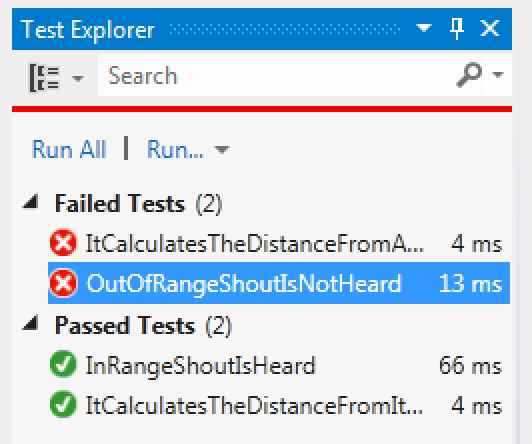
\includegraphics{computer-setup-instructions/expected-test-run}
}
}

If everything goes well, you should see \CUKE{} reporting the following:

\JAVA {
\texttt{2 Scenarios (1 failed, 1 passed)}
\texttt{8 Steps (1 failed, 7 passed)}
}

\RUBY {
\texttt{2 scenarios (1 failed, 1 passed)}
\texttt{8 steps (1 failed, 7 passed)}
}

\JAVASCRIPT {
\texttt{2 scenarios (1 failed, 1 passed)}
\texttt{8 steps (1 failed, 7 passed)}
}

You're now ready to attend the training. Well done! 

If you've run into problems and if the troubleshooting tips below don't
help, please contact us at \texttt{devs@cucumber.io} and we'll do our best to help you out before the training begins.

\chapter*{Troubleshooting}

\section*{Admin rights}

Some of the software will not install if the logged in user doesn't have admin rights.
You need to contact your system administrator if this is the case.

\section*{Proxy configuration}

If some of the software fails to install properly it can be due to missing or incorrect proxy configuration for command line tools.

There are usually two proxy URLs that you need to configure as environment variables: \texttt{HTTP_PROXY} and \texttt{HTTPS_PROXY}.
You may be able to find the proxy URLs in your default web browser's settings. If you can't find them, ask your system administrator.

\subsection*{Windows}

\begin{itemize}
    \item Right-click My Computer, and then click Properties
    \item Click the \texttt{Advanced} tab
    \item Click \texttt{Environment variables}
    \item Click \texttt{New} to add a new user variable
    \begin{itemize}
        \item \texttt{Name}: \texttt{HTTP_PROXY}
        \item \texttt{Value}: \texttt{What the IT department told you}
    \end{itemize}
    \item Click \texttt{New} to add a new user variable
    \begin{itemize}
        \item \texttt{Name}: \texttt{HTTPS_PROXY}
        \item \texttt{Value}: \texttt{What the IT department told you}
    \end{itemize}
\end{itemize}

After you have done this you need to start a new command window to have those environment variables available.

\subsection*{OS X and Linux}

Add the following lines to your \texttt{\textasciitilde/.bash_profile} or similar:

\begin{verbatim}
export HTTP_PROXY=<What the IT department told you>
export HTTPS_PROXY=<What the IT department told you>
\end{verbatim}

After you have done this you need to start a new shell to have those environment variables available.

\end{document}
